\chapter{Umsetzung Teilprojekt SAE}

\section{Datenbank}
Dieser Abschnitt fokussiert sich auf die in der Softwarelösung verwendete Datenbank und deren Modellierung. Für die Software wurde eine SQLite Datenbank verwendet.

In der Software wurde das Entity Framework verwendet um Tabellen und Relationen anhand von zuvor definierten Klassen zu generieren. Dazu wurden 4 Klassen angelegt User, Company, Interest und Address, die dann zu Tabellen automatisch umgewandelt werden. Dabei wird aus Attributen wie z.B. der Name von User eine Spalte mit eben dieser Bezeichnung. Außerdem wird der Datentyp passend zum Attribut gewählt. Relationen werden ebenso erzeugt z.B. wenn ein User eine Adresse besitzt und damit ein Attribut vom Typ Address hat.

\subsection{Datenbankmodell}
Betrachten wir zunächst ein ER-Modell der Datenbank um einen Überblick zu erhalten.

\begin{figure}[h]
	\centering
	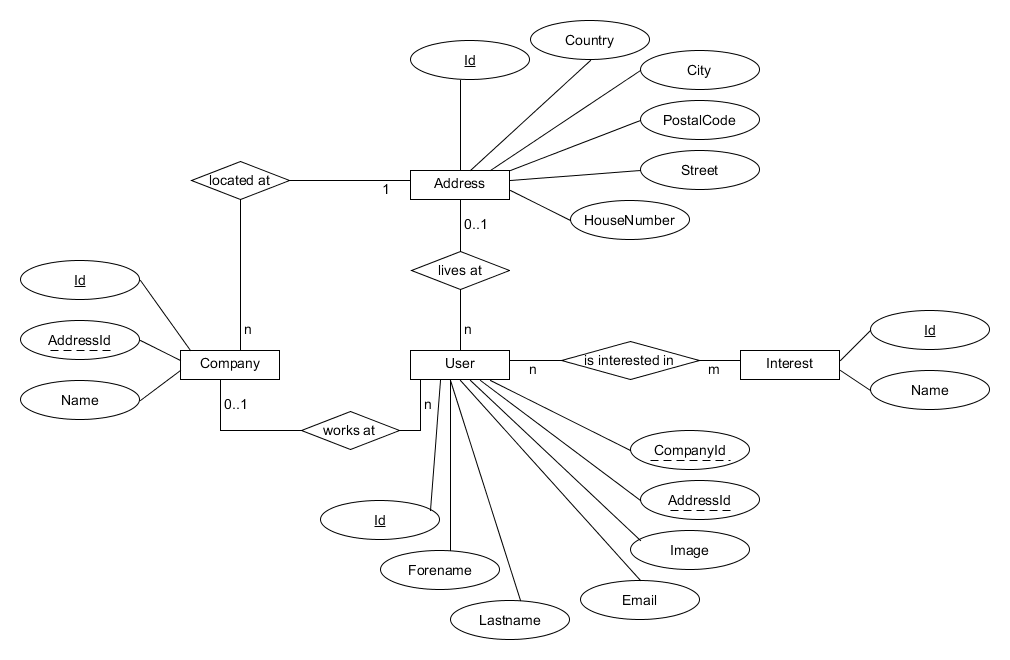
\includegraphics[width=\linewidth]{Images/Projekt_Messe_ERModell2}
	\caption{ER-Modell der Datenbank für die Softwarelösung}
	\label{fig:projektmesseermodell}
\end{figure}

\subsection{Entitäten}
In diesem Abschnitt betrachten wir die Entitäten des ER-Modells und ihre Attribute genauer.

\subsubsection{User}
Die Entität User repräsentiert den Kunden, der seine Daten auf der Messe angegeben hat. Diese Person hat einen Vor- und Nachnamen, Email, Bild, Adresse und eventuell eine Firmenzugehörigkeit. Der Primärschlüssel ist Id, wohingegen AdressId und CompanyId Fremdschlüssel sind.

\subsubsection{Company}
Diese Entität repräsentiert eine Firma, der ein Kunde möglicherweise angehören kann. Sie hat eine Id als Primärschlüssel, einen Namen und eine Adresse mit AddressId als Fremdschlüssel.

\subsubsection{Address}
Die Entität Address hat eine primäre Id, Land, Stadt, Postleitzahl, Straße und Hausnummer.

\subsubsection{Interest}
Eine Interesse hat eine primäre Id und einen Namen.

\subsection{Relationen}

\subsubsection{Company - Address}
Eine Firma hat genau eine Adresse wohingegen an einem Standort auch mehrere Firmen angesiedelt sein können. Dies wird die gezeigte 1:n Relation widergespiegelt. Der Verweise von der Firma auf die Adresse wird mit Hilfe des Fremdschlüssels AddressId gelöst.

\subsubsection{User - Address}
Ein Kunde hat eine oder keine Adresse, wohingegen an einem Ort durchaus mehrere Leute wohnen können. Diese 1:n Relation wird durch den Fremdschlüssel AddressId modelliert.

\subsubsection{User - Company}
Ein Kunde kann Mitarbeiter einer Firma sein, muss es aber nicht und eine Firma kann viele Mitarbeiter haben. Diese 1:n Relation wird durch den Fremdschlüssel CompanyId modelliert.

\subsubsection{User - Interest}
Ein Kunde kann mehrere Interessen haben, aber eine Interesse wie z.B. Reisen kann von vielen Kunden favorisiert werden. Diese n:m Relation wird durch zwei Listen gelöst, wovon sich jeweils eine in der Entität User und Interest befindet.

\newpage
\section{Aufbau und Funktionsweise}
Dieser Abschnitt befasst sich mit dem Aufbau, Architektur und Funktionsweise der Softwarelösung beschrieben mit Hilfe von grafischen Darstellungen mit verschiedenen Diagrammen.

\subsection{Architektur}
\begin{figure}[h]
	\centering
	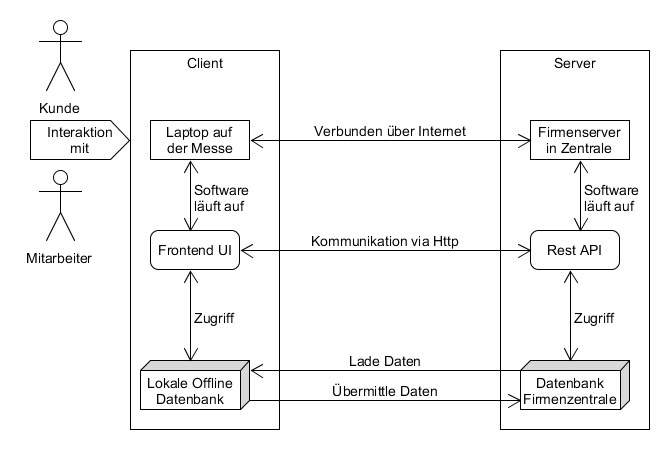
\includegraphics[width=0.8\linewidth]{Images/Projekt_Messe_Architektur}
	\caption{Grafische Darstellung der Architektur}
	\label{fig:projektmessearchitektur}
\end{figure}
Der Aufbau der Softwarelösung ist eine klassische Client-Server-Architektur. Abbildung \ref{fig:projektmessearchitektur} gibt einen Überblick über die beiden Komponenten und ihr Zusammenspiel. 

Der Client befindet sich mit den Mitarbeitern am Messe Stand und ist dort auf den Laptops für die Kunden verfügbar. Dabei handelt es sich um die Frontend UI, die zur Eingabe von Kundendaten und zur Übermittlung an die Firmenserver mit grafische Komponenten dient. Sowohl Kunden als auch Mitarbeiter können den Client bedienen, wobei die Übermittlungsfunktion für Daten lediglich mit Angabe von zuvor registrierten Anmeldedaten benutzt werden kann. Im regulären Betrieb für Kunden befindet sich der Client in einer Art Offline Modus und speichert die Kundendaten in einer lokalen Datenbank ab. Erst nach aktiver Übermittlung an den Firmenserver durch einen Mitarbeiter, werden die Daten zur Firmenzentrale gesendet.

Die Backend Anwendung, eine Rest API, läuft auf den Firmenservern in der Zentrale. Diese wird über das Internet vom Client aus angesteuert, wenn neue Daten durch Mitarbeiter übermittelt werden. Im Gegensatz zur lokalen Client Datenbank, die nur die Daten, des Geräts auf dem diese ausgeführt wird, enthält, sammeln sich in der Datenbank auf dem Firmenserver alle angegebenen Kundendaten an. Zusätzlich werden nach erfolgreicher Übermittlung die Daten vom Client entfernt, um Speicherplatz frei zu machen und Duplikate zu verhindern. Die Mitarbeiter und der Zentrale können im Backend via einer Swagger UI im Browser nach Angabe von validen Anmeldedaten die Kundendaten abfragen.

\newpage
\subsection{USE Case- und Klassen-Diagramme}

\begin{figure}[h]
	\centering
	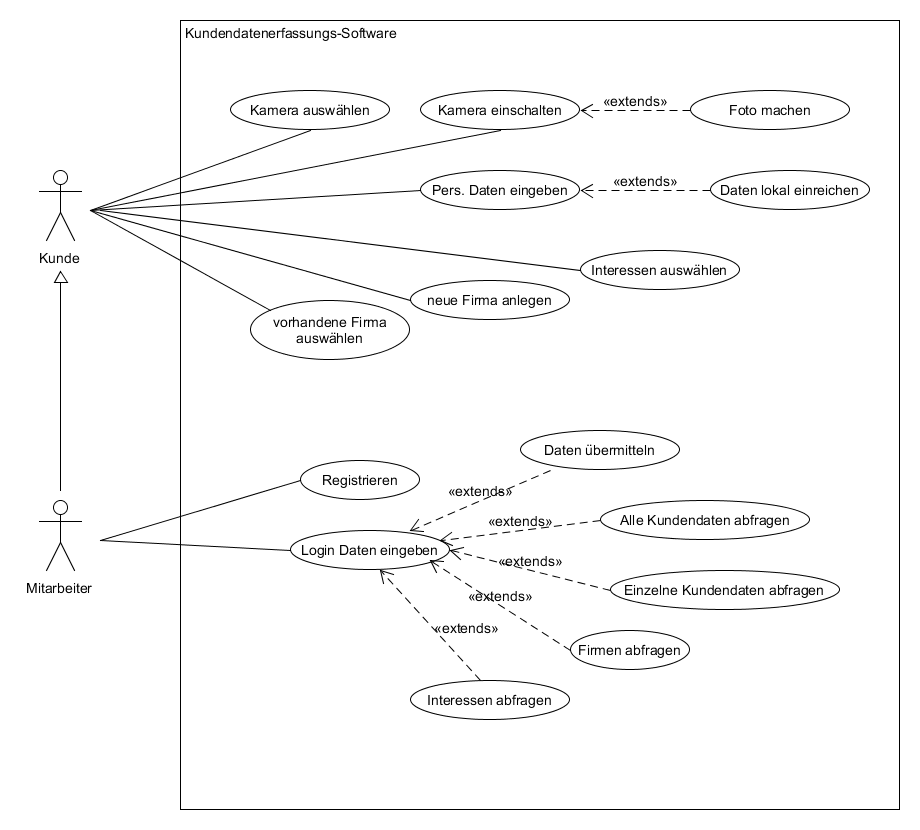
\includegraphics[width=\linewidth]{Images/Projekt_Messe_UseCase2}
	\caption{Use Case Diagramm zur Softwarelösung}
	\label{fig:projektmesseusecase}
\end{figure}

In Abbildung \ref{fig:projektmesseusecase} ist ein Anwendungsfalldiagramm zur Softwarelösung zu sehen. Es gibt zwei Akteure den Kunden und den Mitarbeiter, die verteilt über Frontend UI und Backend Anwendung verschiedene Aktionen durchführen können. Dabei erbt der Mitarbeiter alle Funktionen des Kunden, da dieser auch ohne Angabe von Anmeldedaten alle Aktionen eines Kunden durchführen kann.

\subsubsection{Aktionen eines Kunden}
\begin{itemize}
	\item Kamera auswählen: Mit eine Dropdown Liste kann in der Oberfläche eine Kamera unter all den angeschlossenen gewählt werden. Eine Kamera wird immer als Default ausgewählt sein.
	\item Kamera einschalten: Die ausgewählte Kamera wird eingeschalten und deren Übertragung angezeigt.
	\item Foto machen: Nachdem die Kamera eingeschaltet wurde, kann ein Foto von deren Übertragung gemacht werden.
	\item Persönliche Daten eingeben: Der Kunde kann verschiedene persönliche Daten, wie Name und Anschrift und diversen Textfeldern angeben.
	\item Daten lokal einreichen: Wenn alle notwendigen Daten angegeben wurden, können die Angaben eingereicht und damit lokal gespeichert werden.
	\item Interessen auswählen: Der Kunde kann zwischen verschiedenen vorgegebenen Interessen auswählen und diese per Klick selektieren.
	\item neue Firma anlegen: Wenn von den vorhandenen Firmen keine zusagt, kann eine neue Firma angelegt werden.
	\item Firma auswählen: Der Kunde kann aus verschiedenen angegebenen Firmen eine auswählen.
\end{itemize}

\subsubsection{Aktionen eines Mitarbeiters}
\begin{itemize}
	\item Registrieren: Ein Mitarbeiter kann im Backend neue Anmeldedaten registrieren mit denen er sich später dann in Front- und Backend anmelden kann.
	\item Login Daten eingeben: Der Mitarbeiter kann sowohl im Front- als auch Backend die Anmeldedaten angeben um sich anzumelden.
	\item Daten übermitteln: Nach Angabe von Anmeldedaten kann ein Mitarbeiter die lokal gespeicherten Daten an die Firmenzentrale übermitteln.
	\item Alle Kundendaten abfragen: Ein Mitarbeiter kann nach Angabe von Anmeldedaten im Backend alle Kundendaten abfragen.
	\item Einzelne Kundendaten abfragen: Ein Mitarbeiter kann nach Angabe von Anmeldedaten im Backend einzelne Kundendaten spezifisch abfragen.
	\item Firmen abfragen: Ein Mitarbeiter kann nach Angabe von Anmeldedaten im Backend die Firmen abfragen.
	\item Interessen abfragen: Ein Mitarbeiter kann nach Angabe von Anmeldedaten im Backend die Interessen abfragen.
\end{itemize}
\newpage

\begin{figure}[h]
	\centering
	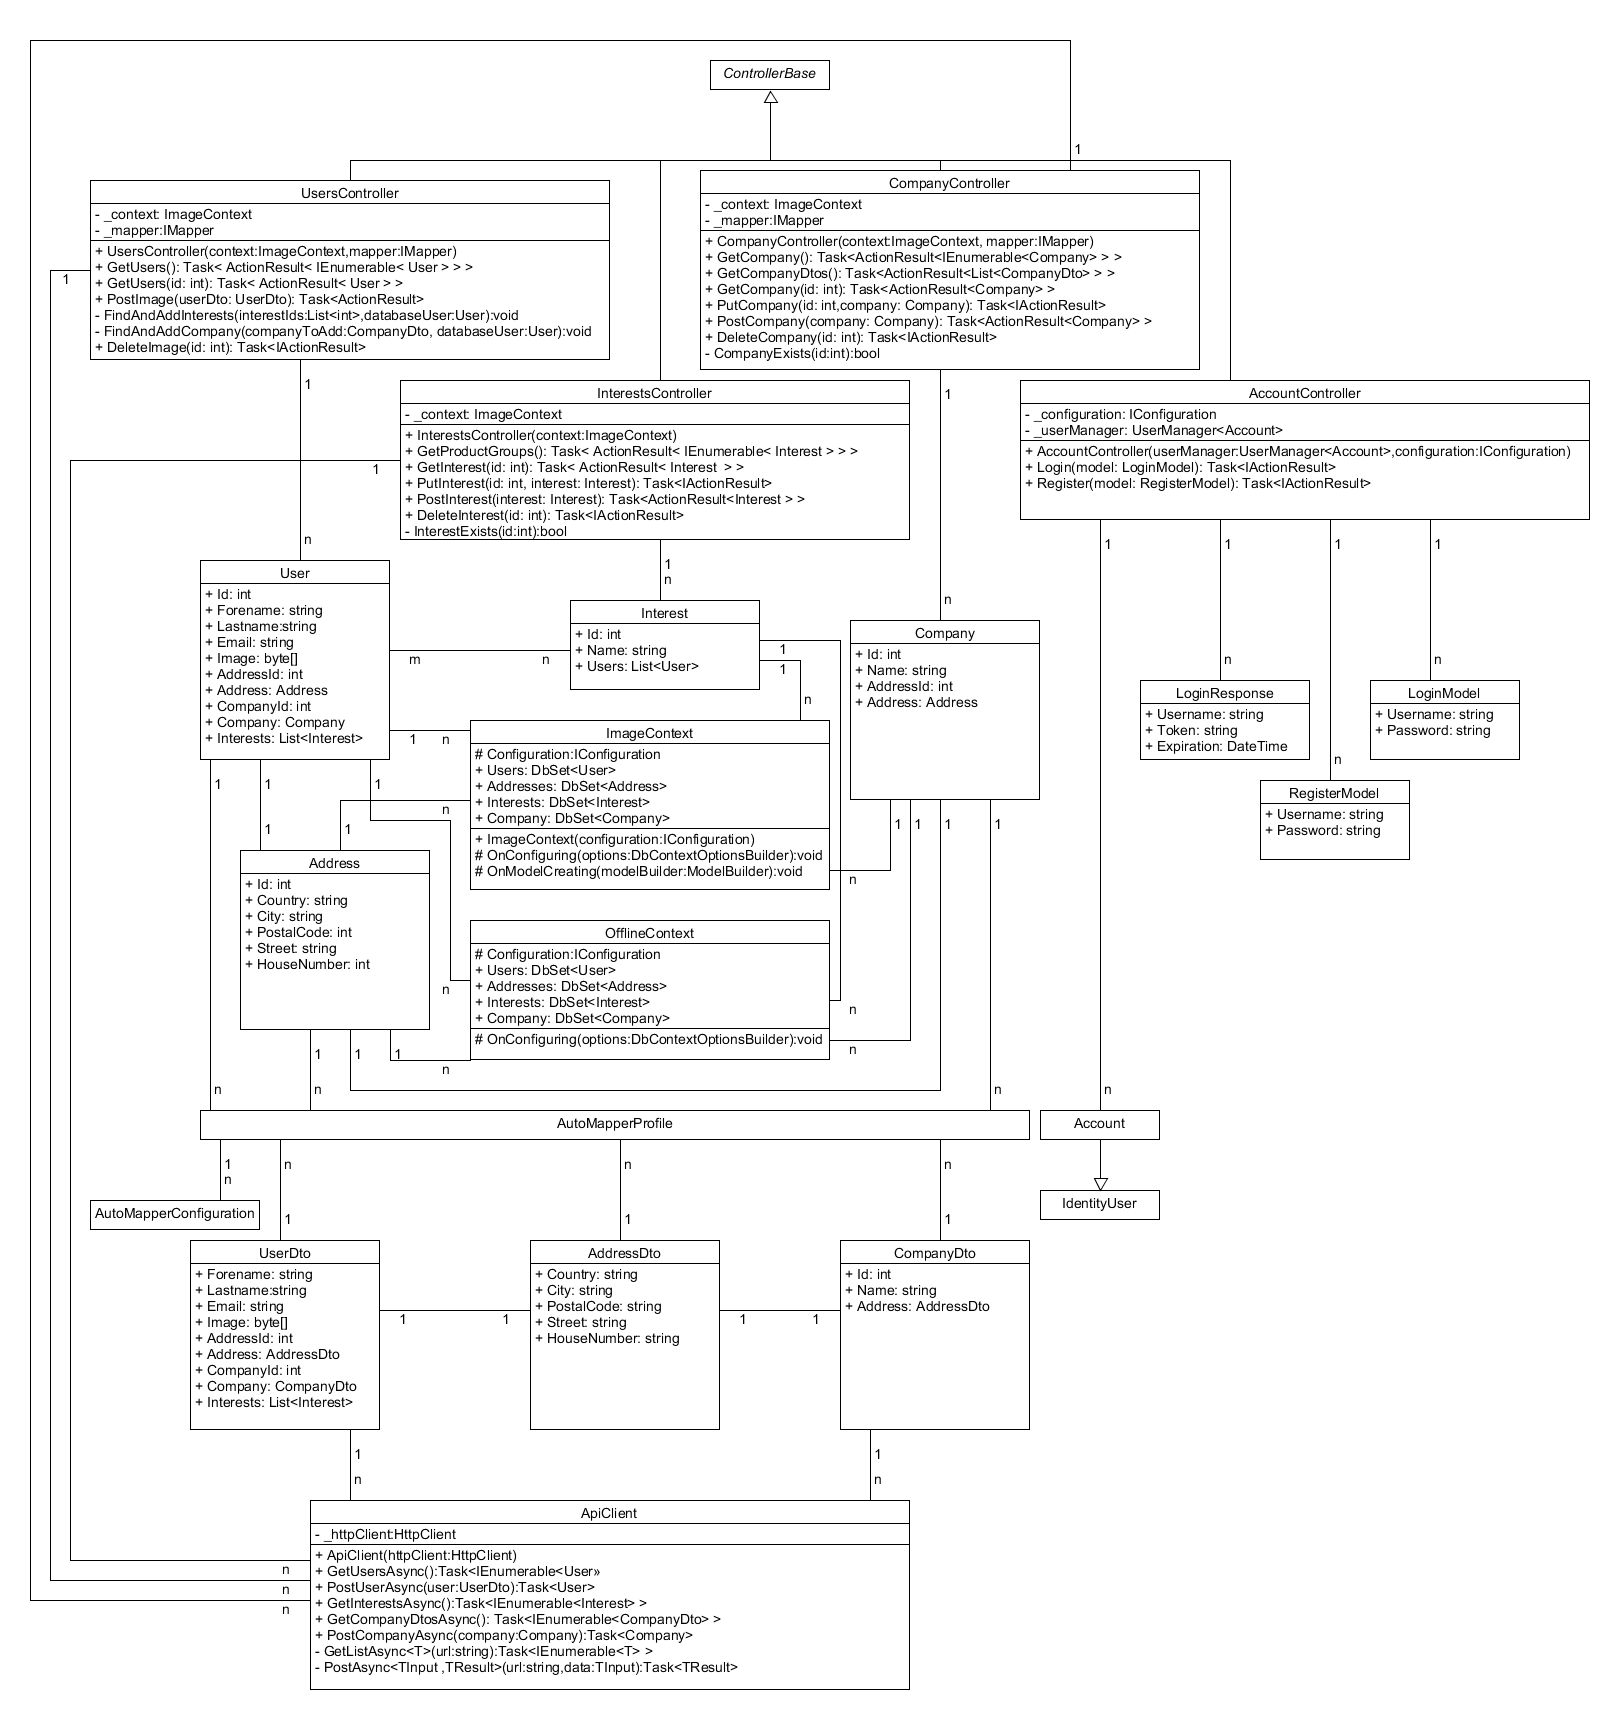
\includegraphics[width=1.1\linewidth]{Images/Projekt_Messe_Class2}
	\caption{Klassen-Diagramm zur Softwarelösung}
	\label{fig:projektmesseclass}
\end{figure}

In Abbildung \ref{fig:projektmesseclass} ist ein Klassendiagramm zur Softwarelösung zu sehen. Im oberen Bereich des Diagramms befinden sich vier Controller Klassen. Diese beinhalten die Http Methoden, wie Get oder Post, die als Rest Api nach außen zum Aufrufen gerichtet sind. Dabei befasst sich UserController mit allen Aktionen rund um die Kundendaten, CompanyController mit den Firmen, zu denen ein Kunde gehören kann, InterestsController mit den Interessen, die Kunden haben können und AccountController mit den Mitarbeiteraccounts, die zum erfolgreichen Anmelden benötigt werden um spezifische Funktionen ausführen zu können.

Im Zentrum des Diagramms sind zum einen die Modellklassen der einzelnen Entitäten User, Interest, Company und Address, wie sie schon im Abschnitt zur Datenbankmodellierung aufgetreten sind. Außerdem befinden sich dort zwei Datenbank Kontext Klassen, ImageContext und OffloneContext. Der Erste Kontext ist die Datenbank auf Seite der Firmenzentrale. Der Zweite ist die lokale Datenbank auf den Clients, welche genutzt wird um die Kundendaten lokal zu speichern, damit kurzzeitige Internetausfälle bei Datenübertragungen umgangen werden. Mit Hilfe der Anmeldedaten eines Mitarbeiter können die lokalen Daten dann zur Firmenzentrale übertragen werden. Beide Datenbankkontext sind gleich aufgebaut, mit je einem DBSet zu allen vier Entitäten.

Im unteren Bereich des Diagramms haben wir zum einen den AutoMapper und die DTOs (Data Transfer Object) und zum anderen den ApiClient. Die ersten beiden werden genutzt um die Daten von den lokalen Datenbanken in DTOs umzuwandeln damit die Informationen dann in diesem Format an die Firmenzentrale geschickt wird. Im Firmenserver werden die DTOs dann wieder in die entsprechenden Entitäten umgemapped und in die dort ansässige Datenbank gespeichert. Der ApiClient wird auf Client Seite verwendet um alle Anfragen an die verschiedenen Teile der API (User, Company, Interest oder Account) zu bündeln und zu vereinfachen.

\subsection{Prerequisites: Bibliotheken und Komponenten}
Sowohl Frontend als auch Backend Anwendungen sind auf .NET 6.0 aufgebaut. Ebenso verwenden beide Anwendungen Automapper (12.0.1), \\ Microsoft.EntityFrameworkCore.Design (6.0.25) und \\ Microsoft.EntityFrameworkCore.Sqlite (6.0.25). Das Backend ist eine ASP.Net API und verwendet zusätzlich noch Microsoft.AspNetCore.Authentication.JwtBearer (6.0.25) und Microsoft.AspNetCore.Identity.EntityFrameworkCore (6.0.25). Das Frontend ist eine Windows Forms Anwendung und verwendet zusätzlich AForge (2.2.5)

\newpage
\subsection{Inbetriebnahme vor Ort}
Nachdem die vier Laptops vor Ort mit dem Netzwerk verbunden wurden, muss die Frontend Software von den Mitarbeitern gestartet werden. Bei der Auswahl der Laptops muss zuvor darauf geachtet werden, dass diese eine Webcam besitzen, oder es werden zusätzliche Webcams mitgebracht, die jetzt vor Start der Anwendung an die Laptops angeschlossen werden müssen. Nachdem die Anwendung gestartet ist öffnet sich ein Fenster wie in Abbildung \ref{fig:projektmesseloginscreen} zu sehen.

\begin{figure}[h]
	\centering
	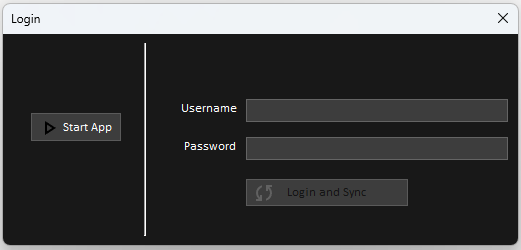
\includegraphics[width=0.7\linewidth]{Images/LoginScreen}
	\caption{Login Bildschirm der Frontend Anwendung}
	\label{fig:projektmesseloginscreen}
\end{figure}

Die Mitarbeiter sollten initial einmal ihre Anmeldedaten eingeben und den Button ''Login and Sync'' drücken um die lokale Datenbank mit der aus der Firmenzentrale zu synchronisieren. Damit wird gewährleistet, dass Interessen oder Firmen, die bereits in der Datenbank der Firmenzentrale hinterlegt wurden, auch lokal für die Kunden zur Auswahl verfügbar sind. Anschließend nachdem die Synchronisation abgeschlossen ist öffnet sich automatisch das nächste Fenster (siehe Abbildung \ref{fig:projektmessemainscreen}).

\begin{figure}[h]
	\centering
	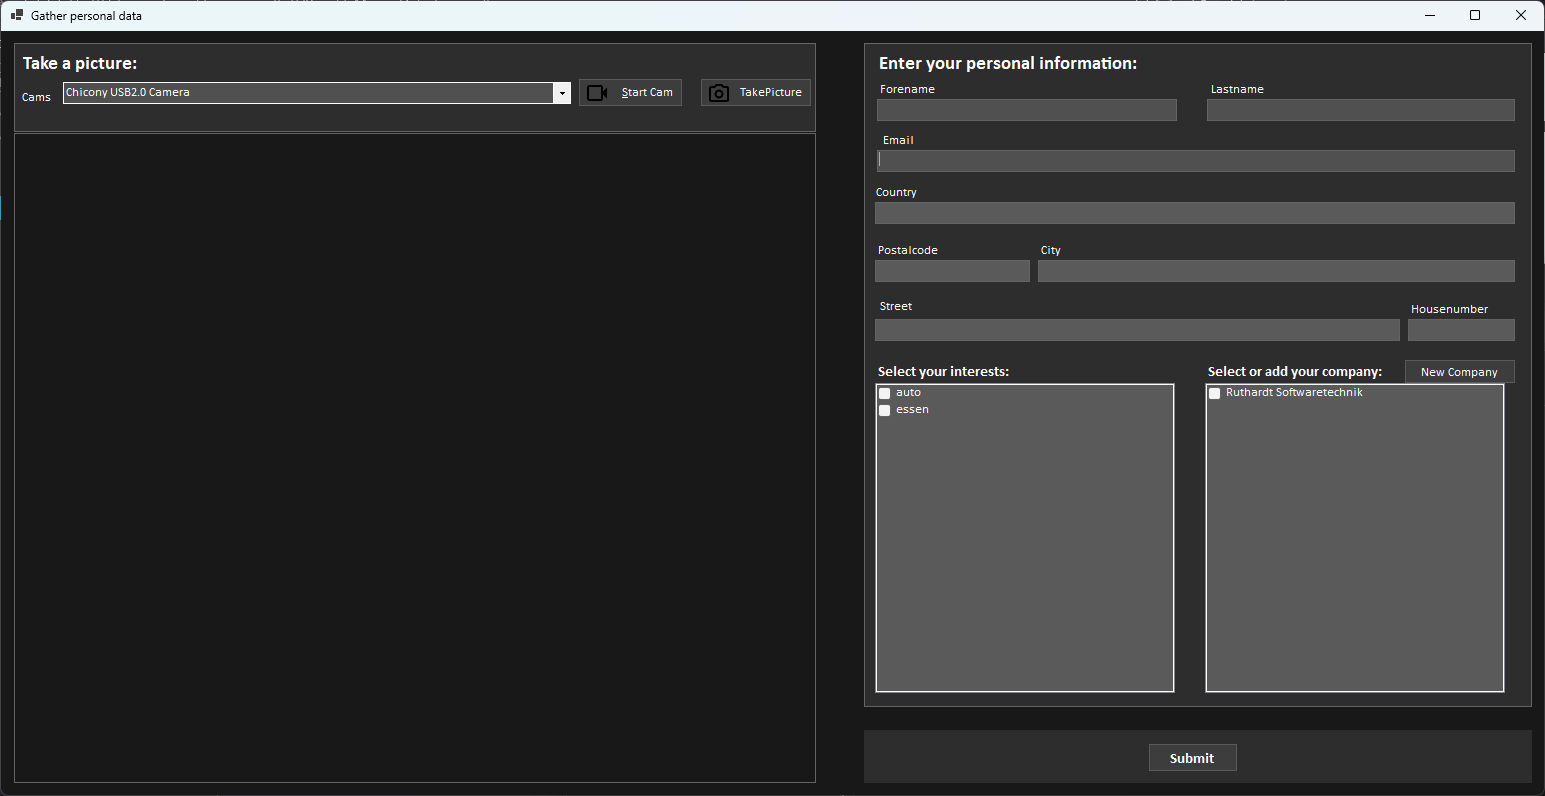
\includegraphics[width=0.9\linewidth]{Images/Hauptbildschirm}
	\caption{Hauptbildschirm der Frontend Anwendung}
	\label{fig:projektmessemainscreen}
\end{figure}

Ein Mitarbeiter sollte im oben links befindlichen Dropdown Menü, die Webcam auswählen, die gewünscht wird und auf den Button ''Start Cam'' drücken um die Kamera zu starten. Jetzt ist die Anwendung einsatzbereit und kann von Kunden genutzt werden.
\newpage
\subsection{Technische Beschreibung der WebCam Anbindung}
Um die Aufnahme der Webcam innerhalb der Frontend Anwendung anzuzeigen wird eine Picturebox verwendet, deren Image Attribute auf den Wert des aktuellen Frame der Webcam gesetzt wird. 
Für die Anbindung der Webcam wird das AFroge Paket verwendet. Zuerst wird wenn die Form des Hauptbildschirms geladen wird alle VideoInputDevices in eine Collection geladen und dem Dropdown Menü hinztugefügt, damit diese zur Auswahl für den Anwendet stehen (siehe Abbildung \ref{fig:projektmessewebcam1}).

\begin{figure}[h]
	\centering
	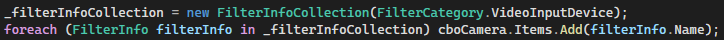
\includegraphics[width=0.9\linewidth]{Images/Projekt_Messe_Webcam1}
	\caption{Collection von VideoInputDevices}
	\label{fig:projektmessewebcam1}
\end{figure}

Wenn nun der ''Start Cam'' Button gedrückt wird, dann wird ein neues VideoCaptureDevice instanziiert anhand der aus dem Dropdown Menü ausgewählten Kamera. Anschließend wird dem NewFrame Event des neuen Objekts eine Methode zugewiesen, die den Frame eines neuen Frame Events eines Videodevices klont. Dieser wird schließlich im UI Thread dem Image der Picturebox zugewiesen (vgl. Abbildung \ref{fig:projektmessewebcam2}).

\begin{figure}[h]
	\centering
	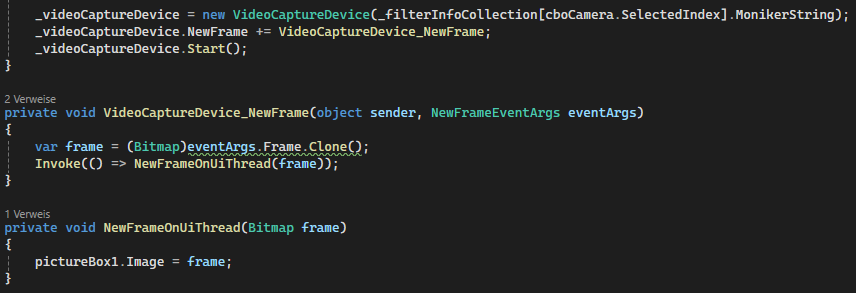
\includegraphics[width=0.9\linewidth]{Images/Projekt_Messe_Webcam2}
	\caption{Starten der Kamera und neuer Frame für Picturebox}
	\label{fig:projektmessewebcam2}
\end{figure}

\newpage
\subsection{Anleitung Bedienung durch den Kunden}
Der Kunde tritt an den Laptop heran und sieht den Hauptbildschirm wie in Abbildung \ref{fig:projektmessemainscreen} zu sehen. Nun muss dieser auf der rechten Seite die persönlichen Daten angeben und kann Interessen auswählen oder eine Firma wo der Kunde Mitarbeiter ist. Dann kann der Kunde noch auf ''Take Picture'' klicken um eine Foto der aktuellen Bilds der Webcam zu machen, damit auch sein Foto gespeichert werden kann. Wenn alle Daten zur Zufriedenheit angegeben wurden und das Fotos ebenso gefällt, kann der Kunde unten rechts auf ''Submit'' klicken und damit seine Daten speichern.

\subsection{Anleitung Datenabruf und Übermittlung}
\subsubsection{Übermittlung}
Ein Mitarbeiter, der über Anmeldedaten verfügt, kann im Login Bildschirm (vgl. Abbildung \ref{fig:projektmesseloginscreen}) diese eintragen und dann auf ''Login and Sync'' drücken. Damit werden die lokal gespeicherten Daten an die Firmenzentrale gesendet. Es ist zu beachten, dass die auf jedem lokalen Gerät auf der Messe durchgeführt werden muss. Außerdem ist wichtig, dass für diese Aktion eine Internetverbindung bestehen sollte, andernfalls können die Daten nicht erfolgreich an die Zentrale gesendet werden. Da das Versenden und lokal Speichern voneinander entkoppelt ist, sollten die Mitarbeiter darauf achten, die Synchronisation dann durchzuführen wenn sichergestellt werden kann, dass eine Verbindung vorliegt.

\subsubsection{Datenabruf}
Der Datenabruf von bereits an die Zentrale übertragenen Daten, kann dort von Mitarbeitern mit Hilfe der Swagger UI im Browser durchgeführt werden. Dazu muss der Mitarbeiter seine Anmeldedaten bereit halten. Zunächst wird die Login von Account Teil der Api aufgeklappt und auf ''Try it out'' geklickt (vgl. Abbildung \ref{fig:projektmesseswagger1}). Dann wird in die Felder bei username und password wo string steht die Anmeldedaten eingetragen. Dann wird auf ''Execute' gedrückt. 

\begin{figure}[h]
	\centering
	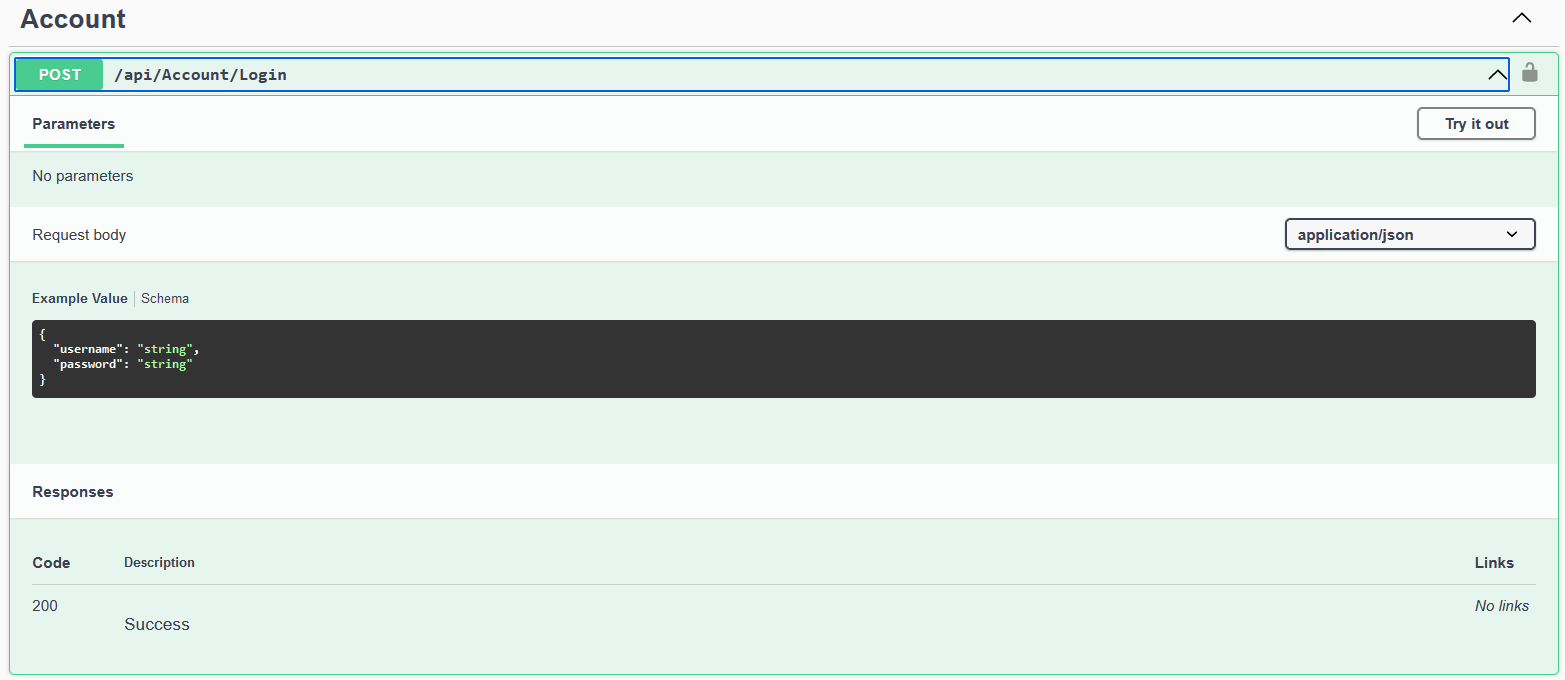
\includegraphics[width=0.9\linewidth]{Images/Projekt_Messe_Swagger1}
	\caption{Login in Swagger UI für Token}
	\label{fig:projektmesseswagger1}
\end{figure}

Unten im Response body befindet sich dann ein Token, diese soll kopiert werden. Dann kann der Login wieder zugeklappt werden. Nun wird oben rechts auf ''Authorize'' geklickt. In das Eingabefeld unter ''Value'' wird zuerst das Wort ''Bearer'' geschrieben und dann das zuvor kopierte Token eingefügt (vgl. Abbildung \ref{fig:projektmesseswagger2}).

\begin{figure}[h]
	\centering
	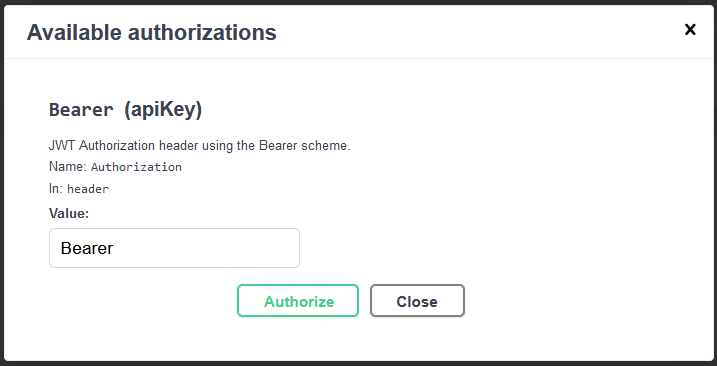
\includegraphics[width=0.7\linewidth]{Images/Projekt_Messe_Swagger2}
	\caption{Login in Swagger UI mit Bearer Token}
	\label{fig:projektmesseswagger2}
\end{figure}

Nachdem der Mitarbeiter nun erfolgreich autorisiert wurde kann dieser alle möglichen Methoden der API nutzen. Um z.B. die in der Datenbank befindlichen Kundendaten abzufragen, gehen wir zum Abschnitt Users und klappen die erste Methode ''Get'' auf. Klicke wieder auf ''Try it out'' und dann auf ''Execute'' (vgl. Abbildung \ref{fig:projektmesseswagger3}). Nun ist im response body der Anfrage alle Kundendaten, mit den jeweiligen Attributen aufgelistet. Unten rechts ist noch die Möglichkeit diese Daten in die Zwischenablage zu kopieren oder gleich die gesamte JSON Ausgabe herunterzuladen.

\begin{figure}[h]
	\centering
	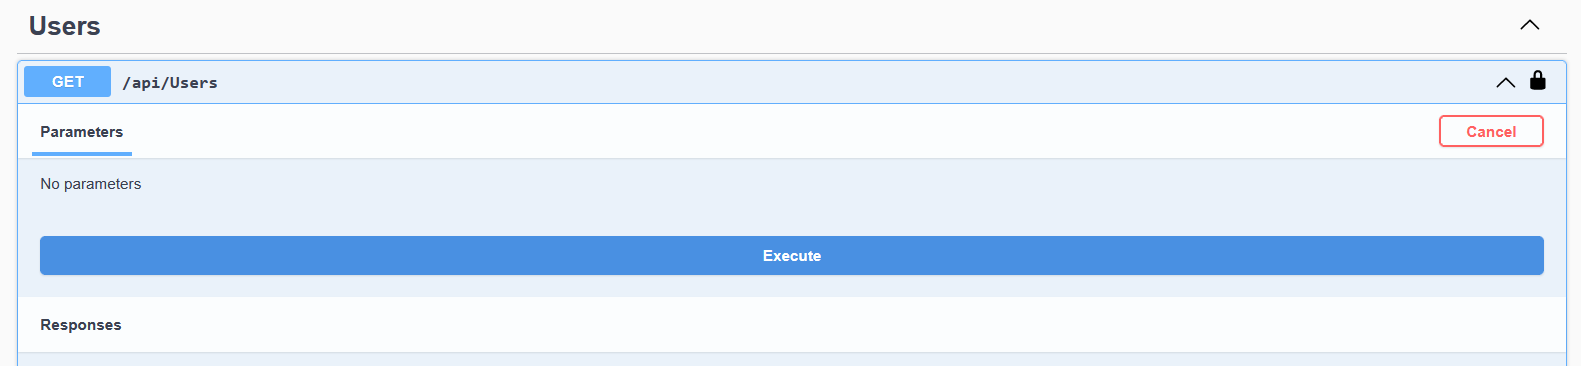
\includegraphics[width=0.9\linewidth]{Images/Projekt_Messe_Swagger3}
	\caption{Abfragen Kundendaten}
	\label{fig:projektmesseswagger3}
\end{figure}


\subsection{Testszenarien}

